\section{Methodology} \label{sec:studysettings}
%We present two studies in this chapter: a quantitative and a qualitative study
%(\hyperref[st:study3]{Studies}~\ref{st:study3} and \ref{st:study4},
%respectively).  

In \hyperref[st:study3]{Study}~\ref{st:study3}, we set out to comparatively
analyze the delivery delay in terms of days (see
\hyperref[def:2]{Definition}~\ref{def:2}) of addressed issues that were shipped
in traditional releases versus the ones that were shipped in rapid releases. In
this section, we provide information about the subject projects, data collection
process, and how we perform the analyses of our study.

\subsection{Subjects}

We choose to study the Firefox project because it offers a unique opportunity to
investigate the impact of shifting from a traditional release cycle to a rapid
release cycle using rich, publicly available ITS and \textit{Version Control
System} (VCS) data. Although other open source projects may have ITS and VCS
data available, they do not provide the opportunity to investigate the
transition between traditional releases and rapid releases. In addition,
comparing different projects that use traditional and rapid releases poses a
great challenge, since one has to distinguish to what extent the results are due
to the release strategy and not due to intricacies of the projects themselves.
Therefore, we highlight that the choice to investigate Firefox is not
accidental, but based on the specific analysis constraints that such data
satisfies, and the very unique nature of such data.

\subsection{Data Collection}\label{ch5:datacollection}

\hyperref[fig:database_construction]{Figure}~\ref{fig:database_construction}
shows an overview of our data collection approach. Each step of the process is
described below.

\begin{figure}[!]
	\centering
	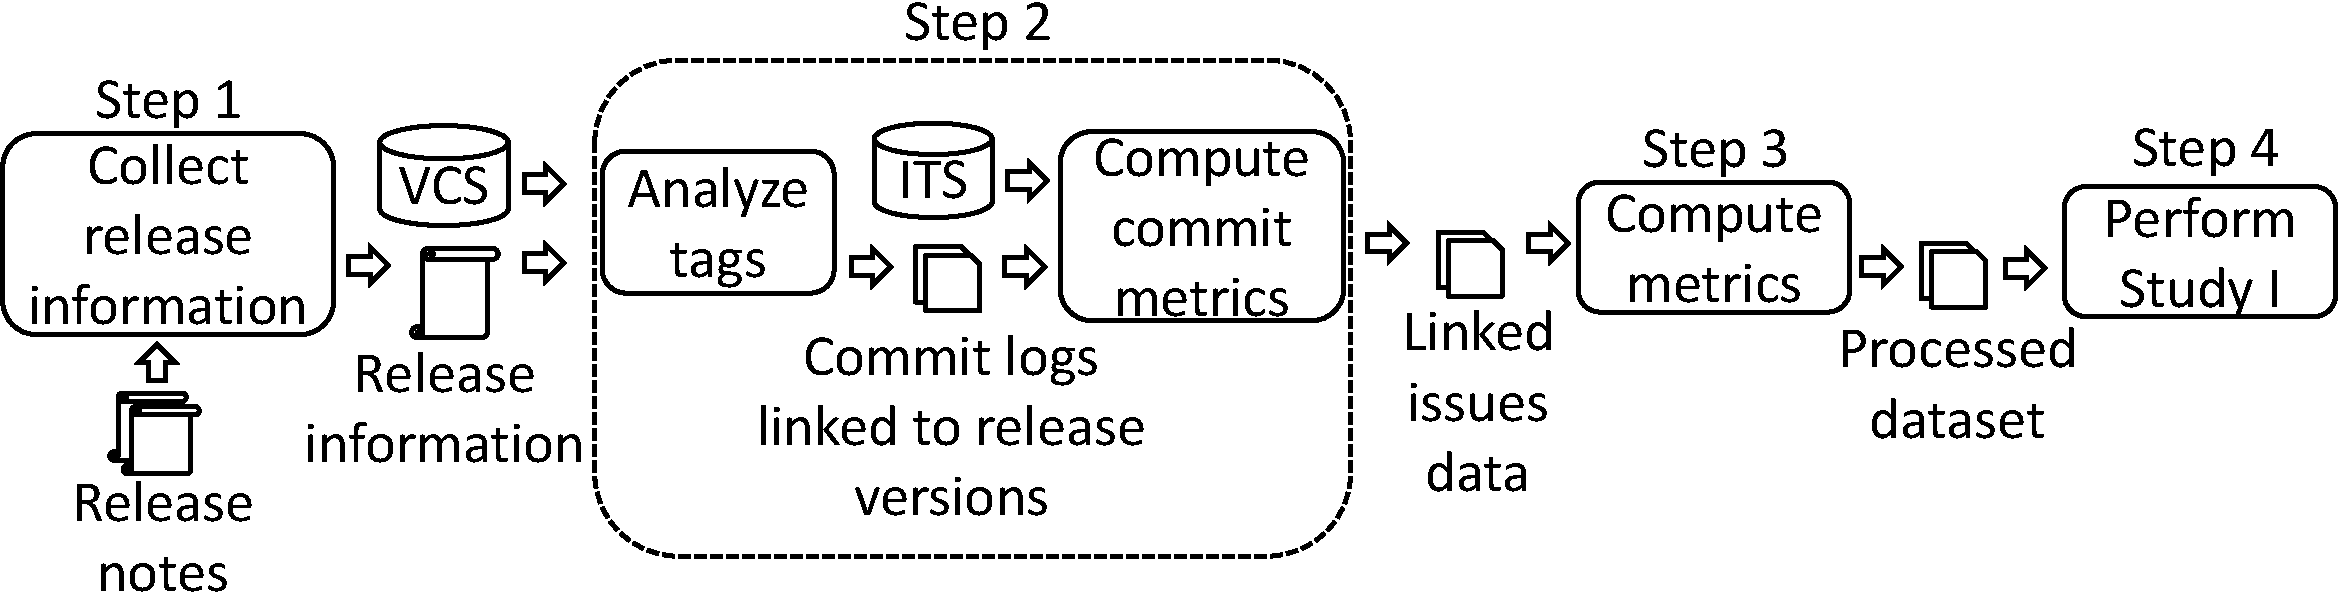
\includegraphics[width=0.90\textwidth,keepaspectratio]
	{chapters/chapter5/figures/database_construction_final.pdf}
	\caption{
		Overview of the process to construct the dataset that is used in
		our \hyperref[st:study3]{Study}~\ref{st:study3}.
	}
	\label{fig:database_construction}
\end{figure}

\begin{table}[!]
	\footnotesize
	\centering
	\caption{The studied traditional and rapid Firefox releases.
	\label{tbl:releases}}
		\begin{tabular}{ccccc}
			\hline 
			\textbf{Strategy} & \textbf{Version range} &
			\textbf{Time period} & \textbf{\# of Majors} &
			\textbf{\# of Minors}\tabularnewline
			\hline 
			\hline 
			Trad. & 1.0 - 4.0 & Sep/2004 - Mar/2012 & 7 & 104\tabularnewline
			\hline 
			Rapid & 5 - 27 & Jun/2011 - Sep/2014 & 23 & 50\tabularnewline
			\hline 
		\end{tabular}%
	%	}
\end{table}

\noindent\textbf{\textit{Step 1: Collect release information.}} We collect the date and
version number of each Firefox release (minor and major releases of each release
strategy) using the Firefox release history
wiki.\smartfoot{\url{https://en.wikipedia.org/wiki/Firefox_release_history}}
\hyperref[tbl:releases]{Table}~\ref{tbl:releases} shows: {\em (i)}the range of versions of releases that we
investigate, {\em (ii)} the investigated time period of each release strategy, and
(iii) the number of major and minor studied releases in each release strategy.\\

\noindent\textbf{\textit{Step 2: Link issues to releases.}} Once we collect the release
information, we use the \textit{tags} within the VCS to link issue IDs to
releases.  First, we analyze the tags that are recorded within the VCS. Since
Firefox migrated from CVS to Mercurial during release 3.5, we collect the tags
of releases 1.0 to 3.0 from CVS, while we collect the tags of releases 3.5 to 27
from
Mercurial.\smartfoot{\url{http://cvsbook.red-bean.com/cvsbook.html}}$^,$\smartfoot{\url{https://mercurial.selenic.com/}}
By analyzing the tags, we extract the commit logs within each tag. The extracted
commit logs are linked to their respective tags. We then parse the commit logs
to collect the issue IDs that are being addressed in the commits. We discard the
following patterns of potential issue IDs that are false positives:

\begin{enumerate}
\item Potential IDs that have less than five digits, since the issue IDs of the
	investigated releases should have at least five digits (2,559 issues
	were discarded).  
\item Commit logs that follow the pattern: ``Bug $<$ID$>$ -
	reftest'' or ``Bug $<$ID$>$ - JavaScript Tests'',
	which refer to tests and not bug fixes (269 issues were
	discarded).  
\item Any potential ID that is the name of a file, \eg
	``159334.js'' (607 issues were discarded).
\end{enumerate}          

We find that all of the remaining IDs match issue IDs that exist in the Firefox
ITS.

Since the commit logs are linked to VCS tags, we are also able to link the
issue IDs found within these commit logs to the releases that correspond to
those tags. For example, since we find the fix for issue 529404 in the commit
log of tag 3.7a1, we link this issue~ID to that release. We also merge together
the data of development releases like 3.7a1 into the nearest minor or major
release. For example, release 3.7a1 would be merged with release 4.0, since it
is the next user-intended release after 3.7a1. In the case that a particular
issue is found in the commit logs of multiple releases, we consider that
particular issue to pertain to the earliest release that contains the last fix
attempt (commit log), since that release is the first one to contain the
complete fix for the issue. Finally, we collect the issue report information
of each remaining issue (\eg opening date, fix date, severity, priority, and
description) using the ITS. Moreover, since the minor-rapid releases are
\textit{off-cycle releases}, in which addressed issues may skip being integrated
into \code{mozilla-central} (\ie NIGHTLY) tags, we manually collect the addressed
issues that were integrated into those releases using the Firefox release notes
(\ie 247 addressed~issues).\smartfoot{\url{https://www.mozilla.org/en-US/firefox/releases/}}
We add the manually collected addressed issues from ESR releases within the rapid
releases data, since they also represent data from a rapid release strategy.\\

\noindent\textbf{\textit{Steps 3 and 4: Compute metrics and perform analyses.}}
We use the data from Step 2 to compute the metrics that we use in our analyses.
We select these metrics (which are described in the
\hyperref[ch5:rq3]{approach for RQ3}) because we suspect that they
share a relationship with delivery delay.

\section{Results} \label{ch4:results}

In this study, we address three research
questions about the shift from a traditional to a rapid release cycle. The
motivation of each research question is detailed below.

\subsection{RQ1: Are addressed issues delivered more quickly in rapid
releases?}\label{ch5:rq1} 

\subsubsection*{RQ1: Motivation} 

Since there is a lack of empirical evidence to indicate that rapid release
cycles deliver addressed issues more quickly than traditional release cycles, we
compare the delivery delay of addressed issues in traditional releases against
the delivery delay in rapid releases in \hyperref[ch5:rq1]{RQ1}.\\

\subsubsection*{RQ1: Approach}

\begin{figure}[t!]
	\centering
	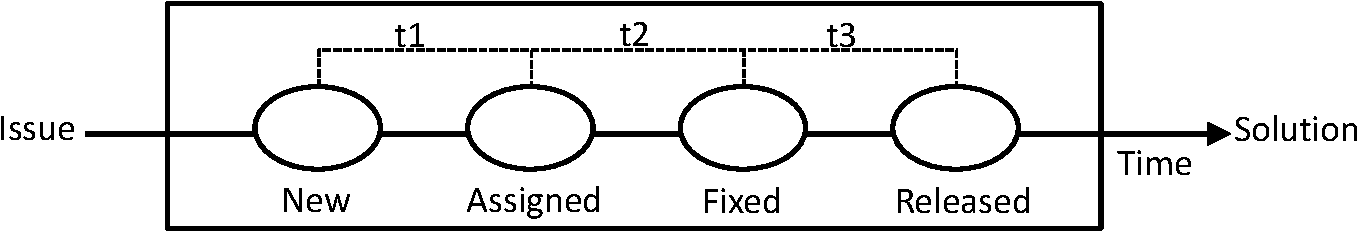
\includegraphics[width=\columnwidth,keepaspectratio]
	{chapters/chapter5/figures/rq1/issue_lifecycle.pdf}
	\caption{A simplified life cycle of an issue.}
	\label{fig:issue_lifecycle}
\end{figure}

\hyperref[fig:issue_lifecycle]{Figure}~\ref{fig:issue_lifecycle} shows a
simplified life cycle of an issue, which includes the triaging phase ({\em t1}),
the fixing phase ({\em t2}), and the integration phase ({\em t3}). We consider
the last RESOLVED-FIXED status as the moment at which a particular issue was
addressed (the fixed state in
\hyperref[fig:issue_lifecycle]{Figure}~\ref{fig:issue_lifecycle}). The
\textit{lifetime} of an issue is composed of all three phases (from \textit{new}
to \textit{released}). For \hyperref[ch5:rq1]{RQ1}, we first observe the lifetime of the issues of
traditional and rapid releases.  Next, we look at the time span of the
\textit{triaging}, \textit{fixing}, and \textit{integration} phases within the
lifetime of an issue.

We use beanplots~\cite{kampstra2008beanplot} to compare the distributions of our
data. The vertical curves of beanplots summarize and compare the distributions
of different datasets (see
\hyperref[fig:delivery_delay]{Figure}~\ref{fig:delivery_delay}). The higher
the frequency of data within a particular value, the thicker the bean is plotted
at that particular value on the $y$ axis. We also use Mann-Whitney-Wilcoxon
(MWW) tests~\cite{wilks2011statistical} and Cliff's delta effect-size
measures~\cite{cliff1993dominance}. MWW tests are non-parametric tests of the
\textit{null hypothesis} that two distributions come from the same population
($\alpha=0.05$). On the other hand, Cliff's delta is a non-parametric
effect-size measure to verify the difference in magnitude of one distribution compared
to another distribution. The higher the value of the Cliff's delta,
the greater the difference of values between distributions. For instance, if we
obtain a significant $p$ value but a small Cliff's delta, this means that
although two distributions do not come from the same population their 
difference is not that large. A positive Cliff's delta indicates how much
larger the values of the first distribution are, while a negative Cliff's delta
indicates the inverse. Finally, we use the \textit{Median Absolute Deviation}
(MAD) \cite{howell2005median,leys2013detecting} as a measure of the variation of
our distributions. The MAD is the median of the \textit{absolute deviations}
from one distribution's median. The higher the MAD, the greater is the variation
of a distribution with respect to its median.

\subsubsection*{RQ1: Results}

\begin{figure}[t!]
	\centering
	\subfloat[Lifetime]{
		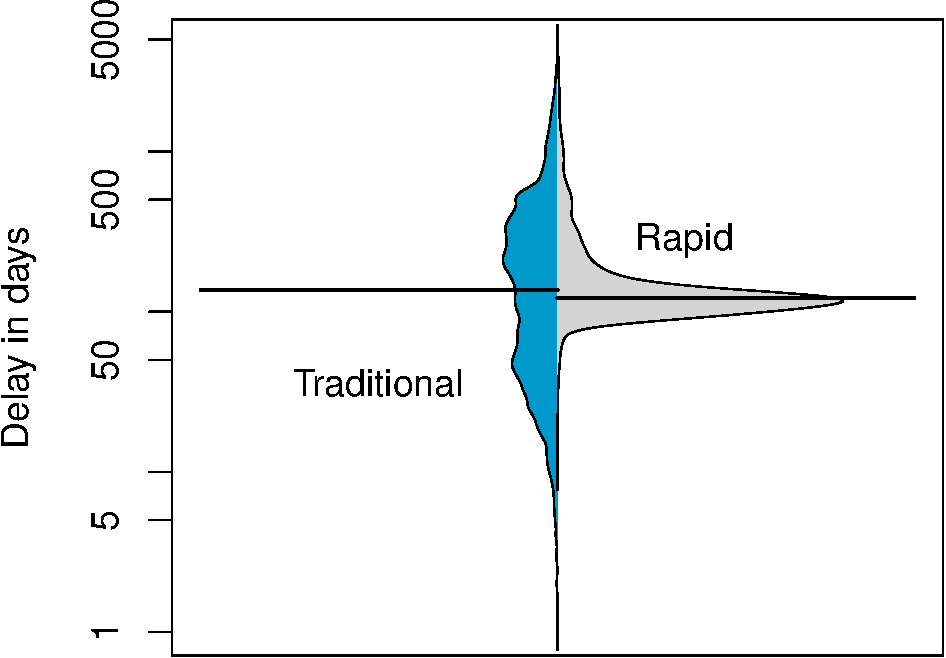
\includegraphics[width=.45\columnwidth,keepaspectratio]
		{chapters/chapter5/figures/rq1/trad-vs-rapid-entire.pdf}
		\label{fig:delivery_delay}
	}
	\subfloat[Triaging phase]{
		\centering
		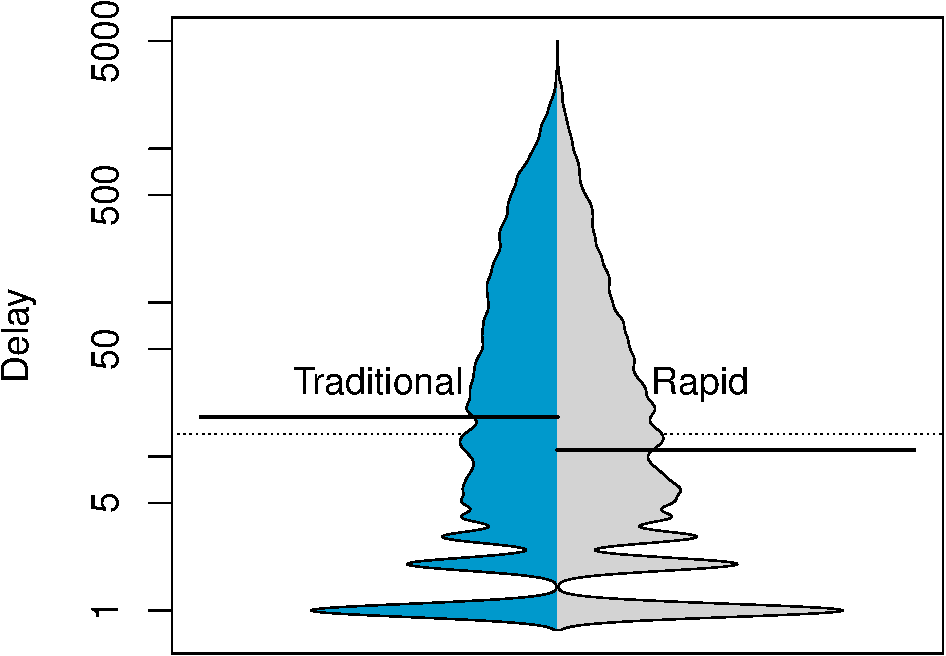
\includegraphics[width=.45\columnwidth,keepaspectratio]
		{chapters/chapter5/figures/rq1/traditional_vs_rapid_triaging.pdf}
		\label{fig:triaging}
	}

	\subfloat[Fixing phase]{
		\centering
		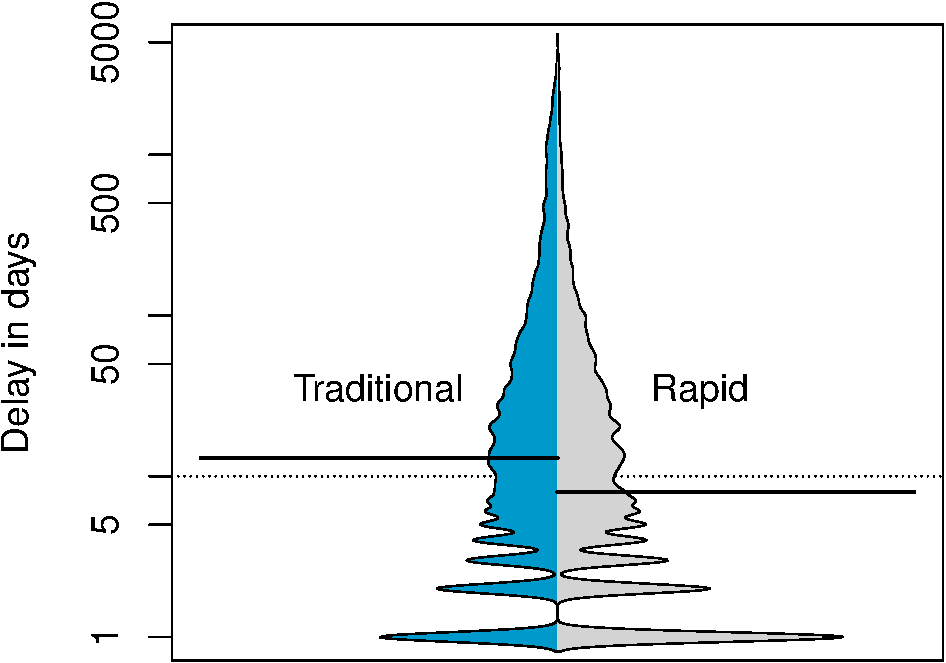
\includegraphics[width=.45\columnwidth,keepaspectratio]
		{chapters/chapter5/figures/rq1/traditional_vs_rapid_fixtime.pdf}
		\label{fig:fixtime}
	}
	\subfloat[Integration phase]{
		\centering
		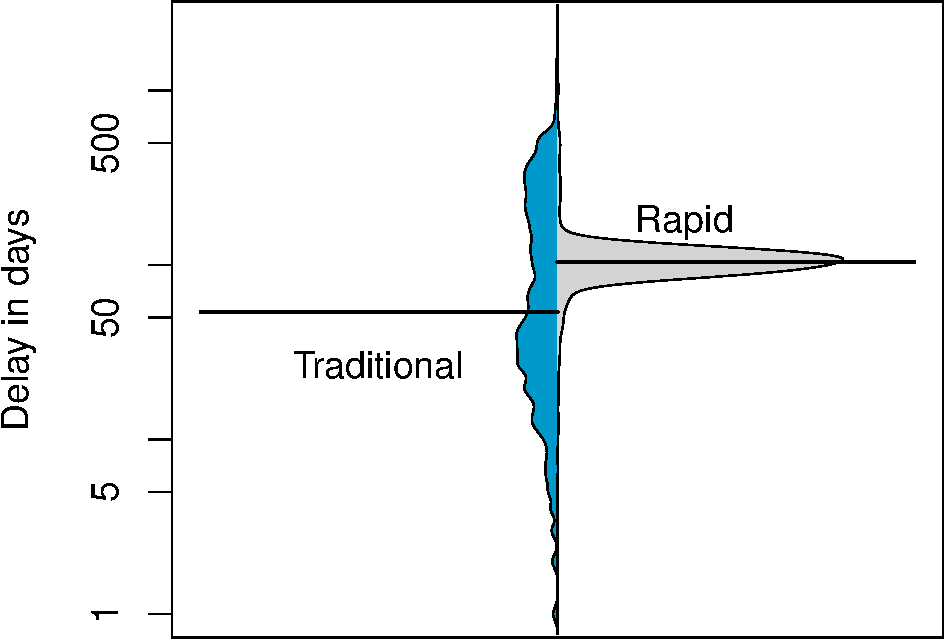
\includegraphics[width=.45\columnwidth,keepaspectratio]
		{chapters/chapter5/figures/rq1/traditional_vs_rapid.pdf}
		\label{fig:traditional_vs_rapid}
	}
	\caption{Time spans of the phases involved in the lifetime of an issue.}
	\label{fig:timespans}
\end{figure}

\noindent\finding{There is no significant difference between traditional and
rapid releases regarding issue lifetime.}{find17}
\hyperref[fig:delivery_delay]{Figure}~\ref{fig:delivery_delay} shows the
distributions of the lifetime of the issues in traditional and rapid releases.
We observe a $p<1.03e^{-14}$ but a $negligible$ difference between the
distributions ($\textit{delta}=0.03$). We also observe that traditional releases
have a greater MAD ($154$ days) than rapid releases ($29$ days), which indicates
that rapid releases are more consistent with respect to the lifetime of the
issues. Our results indicate that the difference in the issues' lifetime between
traditional and rapid releases is not as obvious as one might expect. We then
look at the triaging, fixing, and integration time spans to better understand
the differences between traditional and rapid releases.\\

\noindent\finding{Addressed issues are triaged and fixed more quickly in rapid
releases, but tend to wait for a longer time before being delivered.}{find18}
\hyperref[fig:triaging]{Figures}~\ref{fig:triaging}~,~\ref{fig:fixtime},~and~\ref{fig:traditional_vs_rapid}
show the triaging, fixing, and integration time spans, respectively. We observe
that addressed issues take a median time of 54 days to be integrated into
traditional releases, while taking 104 days (median) to be integrated into rapid
releases. We observe a $p<2.2e^{-16}$ with a $small$ effect-size
($delta=-0.25$).

Regarding fixing time span, an issue takes 6 days (median) to be fixed in rapid
releases, and 9 days (median) in traditional releases. These results are
statistically significant $p<2.2e^{-16}$, but there is only a $negligible$
difference between distributions ($delta=0.13$). 

Our results complement previous research. Khomh~\etal \cite{khomh2012faster}
found that post- and pre-release bugs that are associated with crash reports are
fixed faster in rapid Firefox releases than in traditional releases.
Furthermore, we observe a significant $p<2.2e^{-16}$ but $negligible$ difference
($\textit{delta}=0.11$) between traditional and rapid releases regarding
triaging time. The median triaging time for rapid and traditional releases are
11 and 18 days, respectively.

When we consider both pre-integration phases together (triaging $t1$ plus fixing
$t2$ in \hyperref[fig:issue_lifecycle]{Figure}~\ref{fig:issue_lifecycle}), we
observe that an issue takes $11$ days (median) to triage and address in rapid
releases, while it takes $19$ days (median) in traditional releases. We observe
a $p<2.2e^{-16}$ with a $small$ effect-size ($delta=0.15$). Our results suggest
that even though issues have shorter pre-integration phases in rapid releases,
they remain ``on the shelf'' for a longer time on average.

Finally, we again observe that rapid releases are more consistent than
traditional releases in terms of fixing and delivery rate. Rapid releases
achieve MADs of 9 and 17 days for fixing and delivery, respectively. The values
for traditional releases are 13 and 64 days for fixing and delivery,
respectively.\\ 

\conclusionbox{Although issues are triaged and fixed faster in rapid releases,
they tend to take a longer time to be integrated. However, the delivery rate
of addressed issues is more consistent in rapid releases than in traditional
ones.}

\subsection{RQ2: Why can traditional releases deliver addressed issues
more quickly?}\label{ch5:rq2} 

\subsubsection*{RQ2: Motivation} 

In \hyperref[ch5:rq1]{RQ1}, we surprisingly find that traditional releases tend
to deliver addressed issues more quickly than rapid releases. This result raises
the following question: why can a traditional release strategy, which has a
longer release cycle, deliver addressed issues more quickly than a rapid
release~strategy?\\

\subsubsection*{RQ2: Approach}

In \hyperref[ch5:rq2]{RQ2}, we group traditional and rapid releases into major
and minor releases and study their delivery delays. As in
\hyperref[ch5:rq1]{RQ1}, we also use beanplots~\cite{kampstra2008beanplot}, MWW
tests~\cite{wilks2011statistical}, and Cliff's delta effect-size
measures~\cite{cliff1993dominance} to perform our comparisons.

\subsubsection*{RQ2: Results}

\begin{figure}[t!]
	\centering
	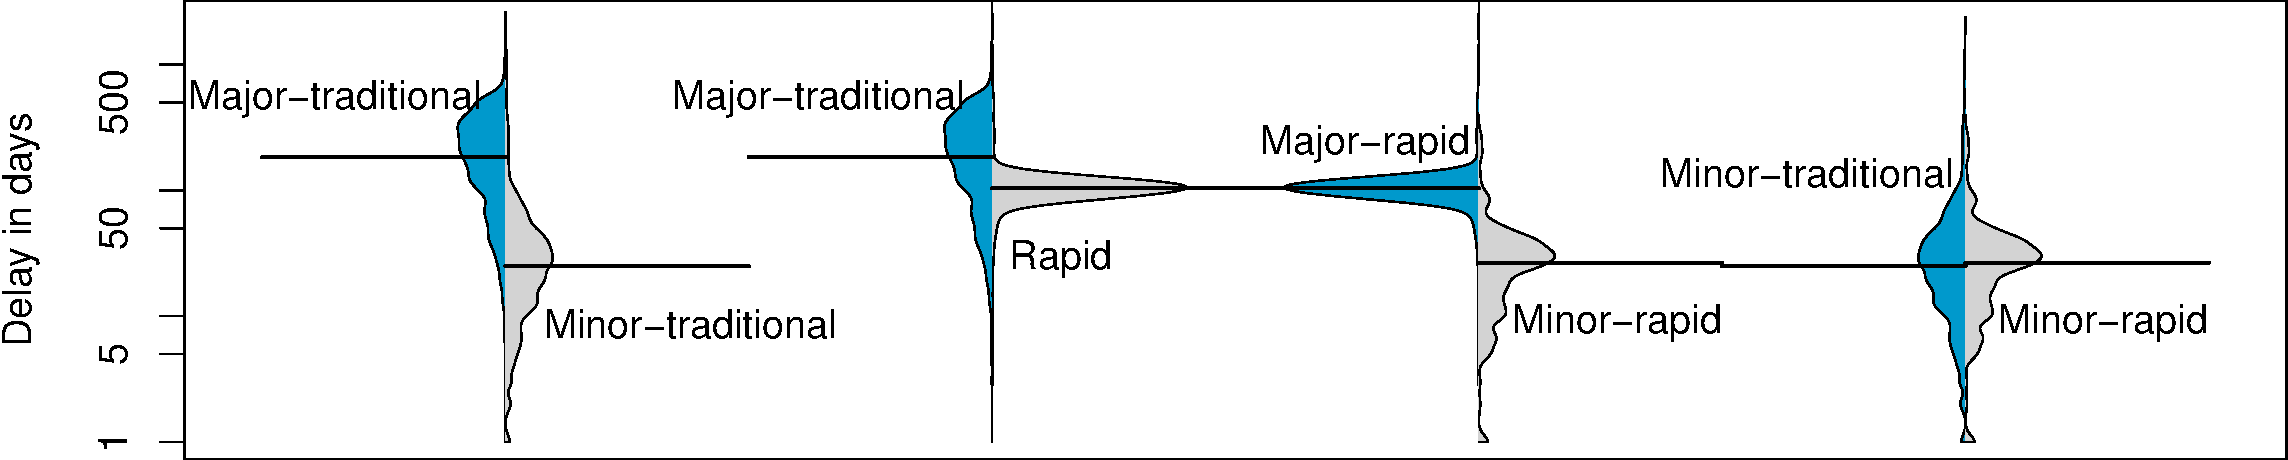
\includegraphics[width=\textwidth,keepaspectratio]
	{chapters/chapter5/figures/rq2/major_vs_minor.pdf}
	\caption{
		Distributions of delivery delay of addressed issues grouped by minor and major
		releases.
	}
	\label{fig:major_vs_minor}
\end{figure}

\begin{sloppypar}
\noindent\finding{Minor-traditional releases tend to have
less delivery delay than major/minor-rapid releases.}{find19}
\hyperref[fig:major_vs_minor]{Figure}~\ref{fig:major_vs_minor} shows the distributions of delivery delay
grouped by (1) \textit{major-traditional vs. minor-traditional}, (2)
\textit{major-traditional vs. rapid}, (3) \textit{major-rapid vs. minor-rapid},
and (4) \textit{minor-traditional vs. minor-rapid}. In the comparison of
\textit{major-traditional vs.  minor-traditional}, we observe that
minor-traditional releases are mainly associated with shorter delivery delay.
Furthermore, in the comparison \textit{major-traditional vs. rapid}, rapid
releases deliver addressed issues more quickly than major-traditional releases
on average ($p<2.2e^{-16}$ with a $medium$ effect-size, \ie  $delta=0.40$). 
\end{sloppypar}

The Firefox rapid release cycle includes ESR releases (see
\hyperref[ch:background]{Chapter}~\ref{ch:background}) and a few minor
stabilization and security releases. These releases also deliver addressed
issues more quickly than major-rapid releases (\textit{major-rapid vs.
minor-rapid}) with a $p<2.2e^{-16}$ and a $large$ effect-size, \ie $delta=0.92$.
Furthermore, we do not observe a statistically significant difference between
distributions in the comparison of \textit{minor-traditional vs. minor-rapid}
($p=0.68$).

Minor-traditional releases have the lowest delivery delay (median of 25
days). This is likely because they are more focused on a particular set of
issues that, once addressed, should be released immediately. For example, the
release history documentation of Firefox shows that minor releases are usually
related to stability and security
issues.\smartfoot{\url{https://www.mozilla.org/en-US/firefox/releases/}}\\

\begin{figure}[t!]
	\centering
	\subfloat[Only Major]{           
		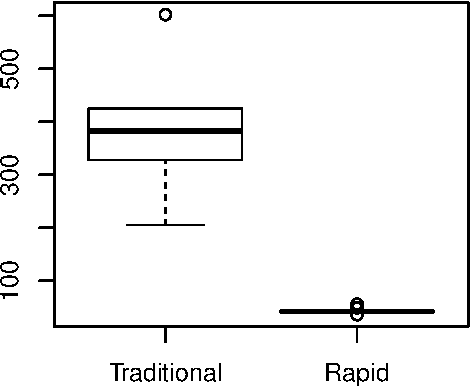
\includegraphics[width=0.45\columnwidth,keepaspectratio]
		{chapters/chapter5/figures/releases/majorreleases_length.pdf}
		\label{fig:majorreleases_length}
	}
	\subfloat[Major and Minor]{
		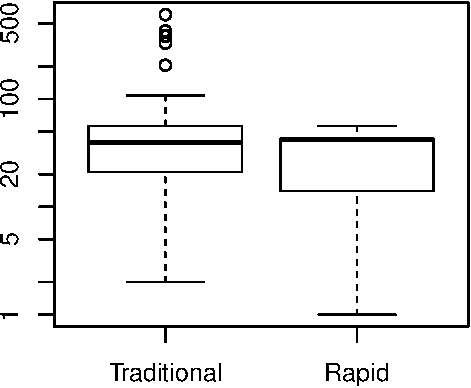
\includegraphics[width=0.45\columnwidth,keepaspectratio]
		{chapters/chapter5/figures/releases/releases_length.pdf}
		\label{fig:releases_length}
	}
	\caption{Release frequency (in days). The outliers in figure~(b)
		represent the major-traditional releases.}
	\label{fig:release_length_analysis}
\end{figure}

\noindent\finding{When considering both minor and major releases, the time span
between traditional and rapid releases are roughly the same.}{find20} Since we
observe that delivery delay is shorter on average in traditional releases, we
also investigate the length of the release cycles to better understand our
previous results (see \hyperref[find19]{Finding}~\ref{find19}).
\hyperref[fig:majorreleases_length]{Figure}~\ref{fig:majorreleases_length} shows
that, at first glance, one may speculate that rapid releases should deliver
addressed issues more quickly because releases are produced more frequently.
However, if we consider both major and minor releases---as shown in
\hyperref[fig:releases_length]{Figure}~\ref{fig:releases_length}---we observe
that both release strategies deliver releases at roughly the same rate on
average (median of $40$ and $42$ days for traditional and rapid releases,
respectively).\\

\conclusionbox{
Minor-traditional releases are one of the main reasons why the traditional
release strategy can deliver addressed issues more quickly than the rapid
release strategy. Furthermore, the lengths of the release cycles are roughly the
same between traditional and rapid releases when both minor and major releases
are considered.
}

\subsection{RQ3: Did the change in the release strategy have an impact on
the characteristics of delayed issues?}\label{ch5:rq3} 

\subsubsection*{RQ3: Motivation}

In \hyperref[ch5:rq1]{RQ1} and \hyperref[ch5:rq2]{RQ2}, we study the differences
between rapid and traditional releases with respect to delivery delay. We find
that although issues tend to be addressed more quickly in rapid releases, they
tend to wait longer to be delivered. We also find that the use of minor releases
is a key reason as to why traditional releases may deliver addressed issues more
quickly. In \hyperref[ch4:rq3]{RQ3}, we investigate what are the characteristics
of each release strategy that are associated with delivery delays. This
important investigation sheds light on what may generate delivery delays in each
release strategy, so that projects are aware of the characteristics of rapid
releases versus traditional releases before choosing to adopt one of these
release strategies. 

\subsubsection*{RQ3: Approach}

\begin{table}[!t]
	\footnotesize
	\caption{Metrics that are used in our explanatory models (Reporter, Resolver,
		and Issue families).
	\label{tbl:factors1}}
	\centering
		\begin{tabular}{rp{2cm}lp{9cm}}
			\hline
			\multicolumn{1}{c}{\textbf{Family}} &
			\multicolumn{1}{c}{\textbf{Metrics}} & \multicolumn{1}{c}{\textbf{Value}} &
			\multicolumn{1}{c}{\textbf{Definition (d)$\vert$Rationale (r)}}
			\\ \hline
			\multicolumn{ 1}{r}{\textbf{Reporter}} & Experience & Numeric & 
			\begin{tabular}{p{8.7cm}}
				\textbf{d:} the number of previously delivered issues that were reported by
				the reporter of a particular addressed issue.  \\ \hline 
				\textbf{r:} The greater the experience of the reporter the
				higher the quality of his/her reports and the
				solution to his/her reports might be delivered
				more quickly~\cite{shihab2010predicting}.
			\end{tabular}
			\\ \cline{2- 4}
			\multicolumn{ 1}{r}{} & Reporter integration & Numeric &
			\begin{tabular}{p{8.7cm}}
				\textbf{d:} The median in days of the previously delivered addressed issues
				that were reported by a particular reporter.
				\\ \hline 
				\textbf{r:} If a particular reporter usually reports issues that are
				delivered quickly, his/her future reported issues might be delivered
				quickly as well.
			\end{tabular}
			\\ \hline
			\multicolumn{ 1}{r}{\textbf{Resolver}} & Experience & Numeric & 
			\begin{tabular}{p{8.7cm}}
				\textbf{d:} the number of previously delivered addressed issues that were
				addressed by the resolver of a particular
				addressed issue. We consider the collaborator
				that changed the status of an issue to
				RESOLVED-FIXED as the resolver of that issue. \\ \hline 
				\textbf{r:} The greater the experience of the resolver, the
				greater the likelihood that his/her code will be
				delivered faster~\cite{shihab2010predicting}.
			\end{tabular}
			\\ \cline{2- 4}
			\multicolumn{ 1}{r}{} & Resolver integration & Numeric &
			\begin{tabular}{p{8.7cm}}
				\textbf{d:} The median in days of the previously delivered addressed issues
				that were addressed by a particular resolver.
				\\ \hline 
				\textbf{r:} If a particular resolver usually address issues that are
				delivered quickly, his/her future addressed issues might be delivered
				quickly as well.
			\end{tabular}
			\\ \hline
			\multicolumn{ 1}{r}{\textbf{Issue}} & Stack trace attached & Boolean &
			\begin{tabular}{p{8.7cm}}
				\textbf{d:} We verify if the issue report has a stack trace attached in its description. \\ \hline 
				\textbf{r:} A stack trace attached may provide useful information regarding
				the cause of the issue, which may quicken the
				delivery of the addressed issue~\cite{schroter2010stack}. 
			\end{tabular}
			\\ \cline{2- 4}
			\multicolumn{ 1}{r}{} & Severity & Nominal &
			\begin{tabular}{p{8.7cm}}
				\textbf{d:} The severity level of the issue report. Issues with higher
				severity levels (\eg blocking) might be delivered faster than other issues.
				\\ \hline 
				\textbf{r:} Panjer observed that the severity of an issue has a large effect
				on its time to be addressed in the Eclipse project~\cite{Panjer2007}.
			\end{tabular}
			\\ \cline{2- 4}
			\multicolumn{ 1}{r}{} & Priority & Nominal &
			\begin{tabular}{p{8.7cm}}
				\textbf{d:} The priority level of the issue report. Issues with higher
				priority levels (\eg P1) might be delivered faster than other issues.
				\\ \hline 
				\textbf{r:} Higher priority issues will likely be delivered before lower
				priority issues.
			\end{tabular}
			\\ \cline{2- 4}
			\multicolumn{ 1}{r}{} & Description size & Numeric &
			\begin{tabular}{p{5.6cm}}
				\textbf{d:} The number of words in the description of the issue. 
				\\ \hline 
				\textbf{r:} Issues that are well described might be more easy to integrate
				than issues that are difficult to understand.
			\end{tabular}
			\\ \hline
		\end{tabular}
\end{table}

\begin{table}[!t]
	\footnotesize
	\caption{Metrics that are used in our explanatory models (Project family).
	\label{tbl:factors2}}
	\centering
		\begin{tabular}{rp{2cm}lp{9cm}}
			\hline
			\multicolumn{1}{c}{\textbf{Family}} &
			\multicolumn{1}{c}{\textbf{Metrics}} & \multicolumn{1}{c}{\textbf{Value}} &
			\multicolumn{1}{c}{\textbf{Definition (d)$\vert$Rationale (r)}}
			\\ \hline
			\multicolumn{ 1}{r}{\textbf{Project}} & Queue rank & Numeric &
			\begin{tabular}{p{8.7cm}}
				\textbf{d:} A rank number that represents the
				moment at which an issue is
				addressed compared to other addressed issues in the backlog. For instance,
				in a backlog that contains $500$ issues, the first addressed issue has
				a rank of~1, while the last addressed issue has
				a rank of 500.
				\\ \hline 
				\textbf{r:} An issue with a high \textit{queue rank} is a recently
				addressed issue. An addressed issue might be delivered faster/slower
				depending of its rank.
			\end{tabular}
			\\ \cline{2- 4}
			\multicolumn{ 1}{r}{} & Cycle queue rank & Numeric &
			\begin{tabular}{p{8.7cm}}
				\textbf{d:} A rank number that represents the
				moment at which an issue is
				addressed compared to other addressed issues of the same release cycle. For
				example, in a release cycle that contains $300$ addressed issues, the first
				addressed issue has a rank of $1$, while the
				last one has a rank of $300$.
				\\ \hline 
				\textbf{r:} An issue with a high \textit{cycle queue rank} is a recently
				addressed issue compared to the others of the same release cycle. An issue
				addressed close to the upcoming release might be delivered faster.
			\end{tabular}
			\\ \cline{2- 4}
			\multicolumn{ 1}{r}{} & Queue position & Numeric &
			\begin{tabular}{p{8.7cm}}
				\textbf{d:} $\frac{\text{queue rank}}{\text{all addressed issues}}$. The
				\textit{queue rank} is divided by all the issues that are addressed by the
				end of the next release. A \textit{queue position} close to 1 indicates that the
				issue was addressed recently compared to others in the backlog.
				\\ \hline 
				\textbf{r:} An addressed issue
				might be delivered faster/slower depending of its position.
			\end{tabular}
			\\ \cline{2- 4}
			\multicolumn{ 1}{r}{} & Cycle queue position & Numeric &
			\begin{tabular}{p{8.7cm}}
				\textbf{d:} $\frac{\text{cycle queue rank}}{\text{addressed issues of the
				current cycle}}$. The \textit{cycle queue rank} is divided by all of the
				addressed issues of the release cycle. A \textit{cycle
				queue position} close to 1 indicates that the issue was addressed recently
				in the release cycle.
				\\ \hline 
				\textbf{r:}  An issue addressed close
				to a upcoming release might be delivered faster. 
			\end{tabular}
			\\ \hline
		\end{tabular}
\end{table}

\begin{table}[!t]
	\footnotesize
	\caption{Metrics that are used in our explanatory models (Process family).
	\label{tbl:factors3}}
	\centering
		\begin{tabular}{rp{2cm}lp{9cm}}
			\hline
			\multicolumn{1}{c}{\textbf{Family}} &
			\multicolumn{1}{c}{\textbf{Metrics}} & \multicolumn{1}{c}{\textbf{Value}} &
			\multicolumn{1}{c}{\textbf{Definition (d)$\vert$Rationale (r)}}
			\\ \hline
			\multicolumn{ 1}{r}{\textbf{Process}} & Number of Impacted Files & Numeric & 
			\begin{tabular}{p{8.7cm}}
				\textbf{d:} The number of files that are linked to an issue report. \\ \hline 
				\textbf{r:} A delivery delay might be
				related to a high number of impacted files 
				because more effort would be required to properly integrate the modifications 
				\cite{Jiang2013}. 
			\end{tabular}
			\\ \cline{ 2- 4}
			\multicolumn{ 1}{r}{} & Churn & Numeric &
			\begin{tabular}{p{8.7cm}}
				\textbf{d:} The sum of added lines plus the sum
				of deleted lines to address the issue.\\ \hline 
				\textbf{r:} A higher churn suggests that a great amount of work was required
				to address the issue, and hence, verifying the impact of integrating the
				modifications may also be difficult~\cite{Jiang2013,Nagappan2005}.
			\end{tabular}
			\\ \cline{2- 4}
			\multicolumn{ 1}{r}{} & Fix time & Numeric &
			\begin{tabular}{p{8.7cm}}
				\textbf{d:} Number of days between the date when
				the issue was
				triaged and the
				date that it was addressed~\cite{Giger2010}. \\ \hline 
				\textbf{r:} If an issue is addressed quickly, it may have a better chance to
				be delivered faster.
			\end{tabular}
			\\ \cline{ 2- 4}
			\multicolumn{ 1}{r}{} & Number of activities & Numeric &
			\begin{tabular}{p{8.7cm}}
				\textbf{d:} An activity is an entry in the issue's history. \\ \hline 
				\textbf{r:} A high number of activities might indicate that much work was
				required to address the issue, which may impact
				the integration and delivery of the
				issue~\cite{Jiang2013}.
			\end{tabular}
			\\ \cline{ 2- 4}
			\multicolumn{ 1}{r}{} & Number of comments & Numeric & 
			\begin{tabular}{p{8.7cm}}
				\textbf{d:} The number of comments of an issue report. \\ \hline 
				\textbf{r:} A large number of comments might indicate the importance of an
				issue or the difficulty to understand it~\cite{Giger2010}, which might
				impact the delivery delay~\cite{Jiang2013}.
			\end{tabular}
			\\ \cline{ 2- 4}
			\multicolumn{ 1}{r}{} & Interval of comments & Numeric &
			\begin{tabular}{p{8.7cm}}
				\textbf{d:} The sum of the time intervals (hour) between
				comments divided by the total number of comments of an issue report. \\ \hline 
				\textbf{r:} A short \textit{interval of comments} indicates that an intense
				discussion took place, which suggests that the issue is important. Hence,
				such an issue may be delivered faster.   
			\end{tabular}
			\\ \cline{ 2- 4}
			\multicolumn{ 1}{r}{} & Number of tosses & Numeric &
			\begin{tabular}{p{8.7cm}}
				\textbf{d:} The number of times that the assignee has changed. \\ \hline 
				\textbf{r:} Changes in the issue assignee might indicate that more than one
				developer have worked on the issue. Such issues may be more difficult to
				integrate, since different expertise from different developers might 
				be required~\cite{Jeong2009,Jiang2013}.  
			\end{tabular}
			\\ \hline
		\end{tabular}
\end{table}

For \hyperref[ch5:rq3]{RQ3}, we build explanatory models (\ie logistic
regression models) for the traditional and rapid releases data using the metrics
that are presented in
\hyperref[tbl:factors1]{Tables}~\ref{tbl:factors1},~\ref{tbl:factors2}, and
\ref{tbl:factors3}. We model our response variable $Y$ as $Y=1$ for addressed
issues that are delayed, \ie had their delivery prevented in at least one
release\cite{costa2014empirical} and $Y=0$ otherwise. Hence, our models are
intended to explain why a given addressed issue has a delayed delivery (\ie
$Y=1$).

\begin{figure}[t!]
	\centering
	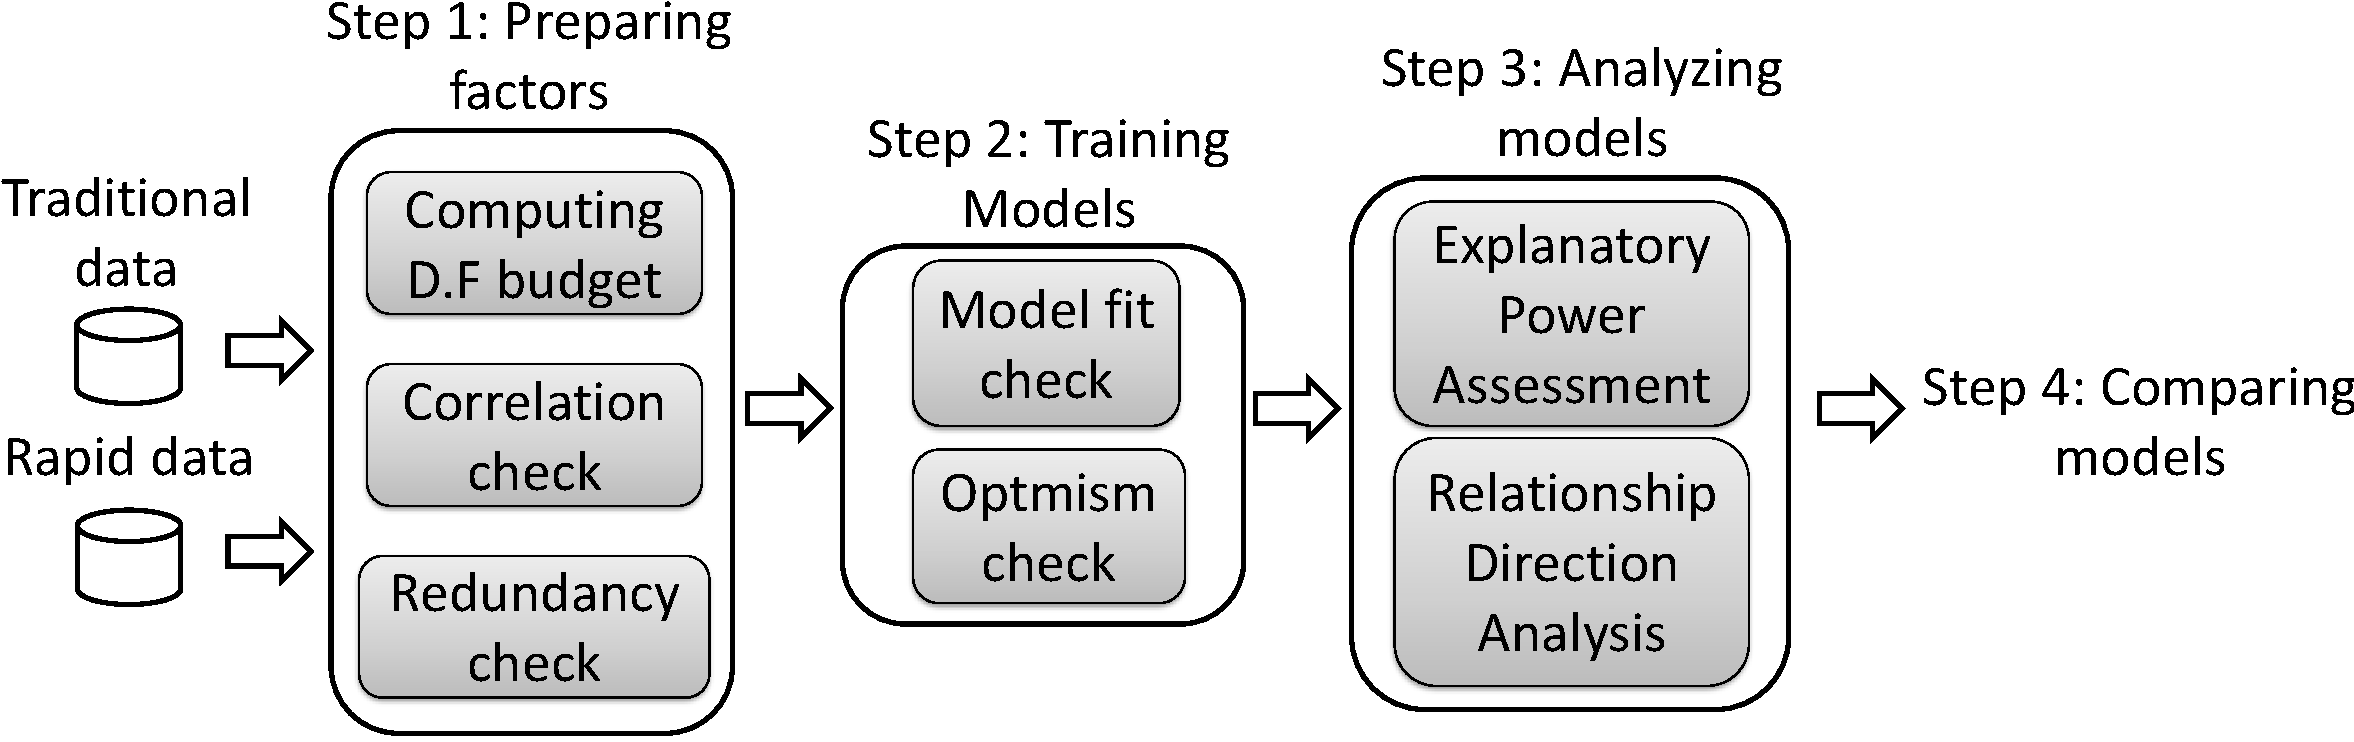
\includegraphics[width=\columnwidth,keepaspectratio]
	{chapters/chapter5/figures/rq3/model_construction.pdf}
	\caption{Overview of the process that we use to build our explanatory models.}
	\label{fig:model_construction}
\end{figure}

We follow the guidelines of Harrell~Jr.~\cite{harrell2001regression} for
building explanatory regression models.
\hyperref[fig:model_construction]{Figure}~\ref{fig:model_construction} provides
an overview of the process that we use to build our models. First, we estimate
the budget of degrees of freedom that we can spend on our models while having a
low risk of overfitting (\ie producing a model that is too specific to the
training data to be useful when applied to other unseen data). Second, we check for
metrics that are highly correlated using Spearman rank correlation tests
$(\rho)$ and we perform a redundancy analysis to remove any redundant metrics
before building our explanatory models. 

We then assess the fit of our models using the ROC area and the Brier score. The
ROC area is used to evaluate the degree of discrimination that is achieved by
a model. The ROC values range between 0 (worst) and 1 (best). An area greater
than 0.5 indicates that the explanatory model outperforms na\"{i}ve random
guessing models. The Brier score is used to evaluate the accuracy of
probabilistic predictions. This score measures the mean squared difference
between the probability of delay assigned by our models for a particular issue
$I$ and the actual outcome of $I$ (\ie whether $I$ is actually delayed or not).
Hence, the lower the Brier score, the more accurate the probabilities that are
produced by a model.

Next, we assess the stability of our models by computing the
\textit{optimism-reduced} ROC area and Brier score~\cite{efron1986biased}. The
optimism of each metric is computed by selecting a bootstrap sample to
fit a model with the same degrees of freedom of the original model. The model
that is trained using the bootstrap sample is applied both on the bootstrap and original
samples (ROC and Brier scores are computed for each sample). The optimism is the
difference in the ROC area and Brier score of the bootstrap sample and original
sample. This process is repeated 1,000 times and the average optimism is
computed. Finally, we obtain the \textit{optimism-reduced} scores by subtracting
the average optimism from the initial ROC area and Brier score
estimates~\cite{efron1986biased}.

We evaluate the impact of each metric on the fitted models using
Wald $\chi^2$ maximum likelihood tests. The larger the $\chi^2$ value, the
larger the impact that a particular metric has on our explanatory models'
performance. We also study the relationship that our metrics 
share with the likelihood of delivery delay. To do so, we plot the change in
the estimated probability of delay against the change in a given metric
while holding the other metrics constant at their median values using the
\code{Predict} function of the \code{rms} package~\cite{harrell2001regression}. 

We also plot nomograms~\cite{iasonos2008build,harrell2001regression} to evaluate
the impact of the metrics in our models. Nomograms are user-friendly charts that
visually represent explanatory models. For instance,
\hyperref[fig:nomogram_trad]{Figure}~\ref{fig:nomogram_trad} shows the nomogram
of the model that we fit for the rapid release data. The higher the number of
points that are assigned to an explanatory metric on the $x$ axis (\eg 100
points are assigned to \textit{comments} in rapid releases), the larger the
effect of that metric in the explanatory model. We compare which metrics are
more important in both traditional and rapid releases in order to better
understand the differences between these release strategies.

\subsubsection*{RQ3: Results}

\begin{sloppypar}
\noindent\finding{Our models achieve a Brier score of 0.05-0.16 and ROC
areas of 0.81-0.83.}{find21}
The models that we fit to traditional releases achieve a Brier score of 0.16 and
an ROC area of 0.83, while the models that we fit to the rapid release data
achieve a Brier score of 0.05 and an ROC area of 0.81. Our models outperform
na\"{i}ve approaches such as random guessing and ZeroR---our ZeroR models
achieve ROC areas of 0.5 and Brier scores of 0.06 and 0.45 for rapid and
traditional releases, respectively. Moreover, the bootstrap-calculated optimism
is less than 0.01 for both the ROC areas and Brier scores of our models. This
result shows that our regression models are stable enough to perform the
statistical inferences that follow.\\

\begin{table}[t]
	\scriptsize
	\begin{center}
		\caption{Overview of the regression model fits. The $\chi^2$ of
		each metric is shown as the proportion in relation to the total
	$\chi^2$ of the model.  \label{tbl:regression_models} }
		%\resizebox{\textwidth}{!}{
			\begin{tabular}{cccc}
			\cline{3-4} 
			\multicolumn{2}{c}{} & 
			Traditional releases &
			Rapid releases 
			\tabularnewline
			\hline 
			\multicolumn{2}{c}{\# of instances} & 
			$34,673$ &
			$37,441$  
			\tabularnewline
			\hline
			\multicolumn{2}{c}{Wald $\chi^2$} & 
			$4,964$ &
			$2,705$  
			\tabularnewline
			\hline 
			\multicolumn{2}{c}{Budgeted Degrees of Freedom} &
			$1033$ & 
			$149$ 
			\tabularnewline
			\hline
			\multicolumn{2}{c}{Degrees of Freedom Spent} &
			$26$ & 
			$25$ 
			\tabularnewline
			%\hline 
			%\hline 
			%&  &  &  
			%\tabularnewline
			\hline 
			\multirow{2}{*}{Reporter experience} & 
			D.F. & 
			$1$ & 
			$1$  
			\tabularnewline 
			& 
			$\chi^2$ & 
			$2^{\ast\ast\ast}$ &  
			$2^{\ast\ast\ast}$ 
			\tabularnewline
			\hline 
			\multirow{2}{*}{Reporter integration} & 
			D.F. & 
			$1$ & 
			$1$  
			\tabularnewline 
			& 
			$\chi^2$ & 
			$5^{\ast\ast\ast}$ &  
			$4^{\ast\ast\ast}$ 
			\tabularnewline
			\hline 
			\multirow{2}{*}{Resolver Experience} & 
			D.F. & 
			$1$ & 
			\multirow{2}{*}{$\oslash$}
			\tabularnewline &
			$\chi^2$ & 
			$1^{\ast\ast\ast}$ &
			\tabularnewline 
			\hline 
			\multirow{2}{*}{Resolver integration} & 
			D.F. & 
			$1$ & 
			$1$  
			\tabularnewline 
			& 
			$\chi^2$ & 
			$2^{\ast\ast\ast}$ &  
			$5^{\ast\ast\ast}$ 
			\tabularnewline
			\hline 
			\multirow{2}{*}{Fix time} & 
			D.F. & 
			1 &
			1  
			\tabularnewline & 
			$\chi^2$ &
			$2^{\ast\ast\ast}$ &
			$8^{\ast\ast\ast}$ 
			\tabularnewline \hline 
			\multirow{2}{*}{Severity} &
			D.F. & 
			$6$ & 
			$6$ 
			\tabularnewline & 
			$\chi^2$ & 
			$1^{\ast\ast\ast}$ &  
			$1^{\ast\ast\ast}$  
			\tabularnewline \hline 
			\multirow{2}{*}{Priority} & 
			D.F. & 
			$5$ & 
			$5$ 
			\tabularnewline & 
			$\chi^2$ & 
			$1^{\ast\ast\ast}$ &  
			$\approx 0$   
			\tabularnewline \hline 
			\multirow{2}{*}{Size of description} & 
			D.F. & 
			$1$ &
			$1$  
			\tabularnewline & 
			$\chi^2$ & 
			$\approx 0$ &
			$1^{\ast\ast\ast}$   
			\tabularnewline \hline 
			\multirow{2}{*}{Stack trace attached} & 
			D.F. & 
			$1$ &
			$1$  
			\tabularnewline & 
			$\chi^2$ & 
			$\approx 0$ &  
			$\approx 0$ 
			\tabularnewline \hline 
			\multirow{2}{*}{Number of files} & 
			D.F. & 
			$1$ & 
			$1$
			\tabularnewline & 
			$\chi^2$ & 
			$1^{\ast\ast\ast}$ &  
			$1^{\ast\ast\ast}$ 
			\tabularnewline \hline 
			\multirow{2}{*}{Number of comments} & 
			D.F. & 
			$1$ &
			$1$ 
			\tabularnewline & 
			$\chi^2$ & 
			$\approx 0^{\ast}$ &  
			$31^{\ast\ast\ast}$  
			\tabularnewline \hline 
			\multirow{2}{*}{Number of tossing} & 
			D.F. & 
			$1$ &
			$1$  
			\tabularnewline & 
			$\chi^2$ & 
			$\approx 0^{\ast\ast\ast}$ &  
			$\approx 0$   
			\tabularnewline \hline 
			\multirow{2}{*}{Number of activities} & 
			D.F. & 
			$1$ &
			$1$  
			\tabularnewline & 
			$\chi^2$ & 
			$1^{\ast\ast\ast}$ &  
			$3^{\ast\ast\ast}$  
			\tabularnewline \hline 
			\multirow{2}{*}{Interval of comments} & 
			D.F. & 
			\multirow{2}{*}{$\oslash$} &
			\multirow{2}{*}{$\oslash$}  
			\tabularnewline &
			$\chi^2$ &
			&
			\tabularnewline \hline 
			\multirow{2}{*}{Code churn} & 
			D.F. & 
			$1$ & 
			$1$  
			\tabularnewline &
			$\chi^2$ &
			$\approx 0$ &  
			$\approx 0$ 
			\tabularnewline \hline 
			\multirow{2}{*}{Queue position} & 
			D.F. & 
			$1$ &             
			$1$
			\tabularnewline & 
			$\chi^2$ & 
			$17^{\ast\ast\ast}$ & 
			$2^{\ast\ast\ast}$
			\tabularnewline \hline 
			\multirow{1}{*}{Queue rank} & 
			D.F. & 
			$1$ & 
			$1$ 
			\tabularnewline &
			$\chi^2$ & 
			$56^{\ast\ast\ast}$ & 
			$14^{\ast\ast\ast}$
			\tabularnewline \hline 
			\multirow{2}{*}{Cycle queue rank} & 
			D.F. & 
			$1$ &
			$1$ 
			\tabularnewline &
			$\chi^2$ & 
			$10^{\ast\ast\ast}$ &
			$28^{\ast\ast\ast}$ 
			\tabularnewline \hline 
			\multirow{2}{*}{Cycle queue position} & 
			D.F. & 
			\multirow{2}{*}{$\oplus$} &
			\multirow{2}{*}{$\oslash$}  
			\tabularnewline &
			$\chi^2$ & 
			&
			\tabularnewline \hline 
		\end{tabular}
%	}
	\captionsetup{justification=centering}
	\caption*{
		$\oslash$ discarded during correlation analysis \\
		$\oplus$ discarded during redundancy analysis \\
		$\ast$ $p < 0.05$;
		$\ast\ast$ $p < 0.01$;
		$\ast\ast\ast$ $p < 0.001$\\ 
	}
	\end{center}
\end{table}

\noindent\finding{Traditional releases prioritize the delivery
of backlog issues, while rapid releases prioritize the delivery of issues of the
current release cycle.}{find22}
\hyperref[tbl:regression_models]{Table}~\ref{tbl:regression_models} shows the
explanatory power ($\chi^2$) of each metric that we use in our models.  The
\textit{queue rank} metric is the most important metric in the models that we
fit to the traditional release data.  Queue rank measures the moment when an
issue is addressed in the backlog of the project (see
\hyperref[tbl:factors2]{Table}~\ref{tbl:factors2}).
\hyperref[fig:rankposition]{Figure}~\ref{fig:rankposition} shows the
relationship that queue rank shares with delivery delay. Our models reveal that
the addressed issues in traditional releases have a higher likelihood of being
delayed if they are addressed later when compared to other issues in the backlog
of the project.   

\begin{figure}[t]
	\centering
	\subfloat{
		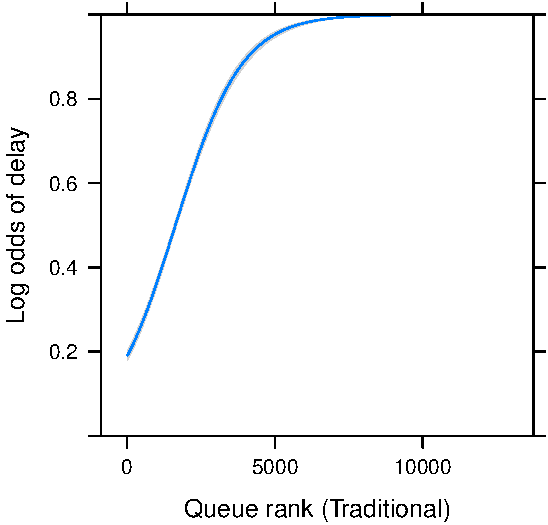
\includegraphics[width=0.43\textwidth,keepaspectratio]
		{chapters/chapter5/figures/rq3/queue_rank.pdf}
		\label{fig:rankposition}
	}
	\subfloat{
		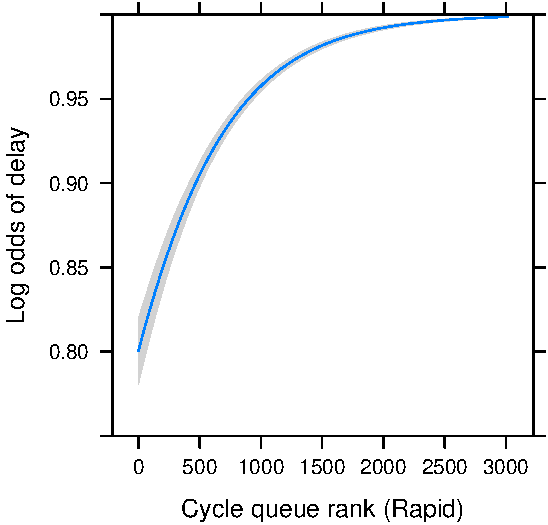
\includegraphics[width=0.43\textwidth,keepaspectratio]
		{chapters/chapter5/figures/rq3/cycle_queue_rank.pdf}
		\label{fig:cycle_rank}
	}

	\subfloat{
		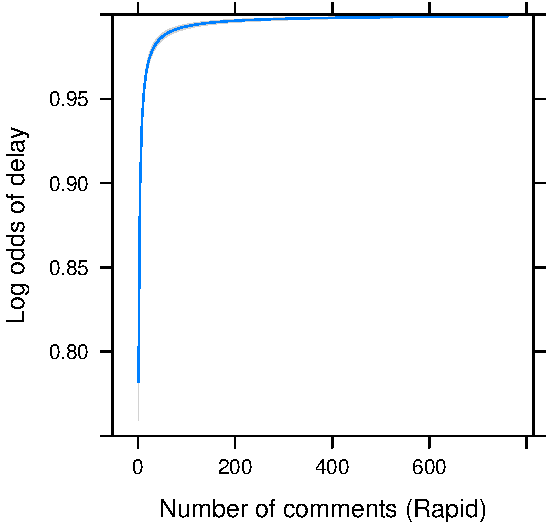
\includegraphics[width=0.43\textwidth,keepaspectratio]
		{chapters/chapter5/figures/rq3/comments.pdf}
		\label{fig:number_comments}
	}
	\caption{The relationship between metrics and delivery delay. The blue
		line shows the values of our model fit, whereas the grey
		area shows the 95\% confidence interval based on models fit to
		1,000 bootstrap samples. The parentheses indicate the
		release strategy to which the metric is related.
	}
\end{figure}

\begin{figure}[!]
	\centering
	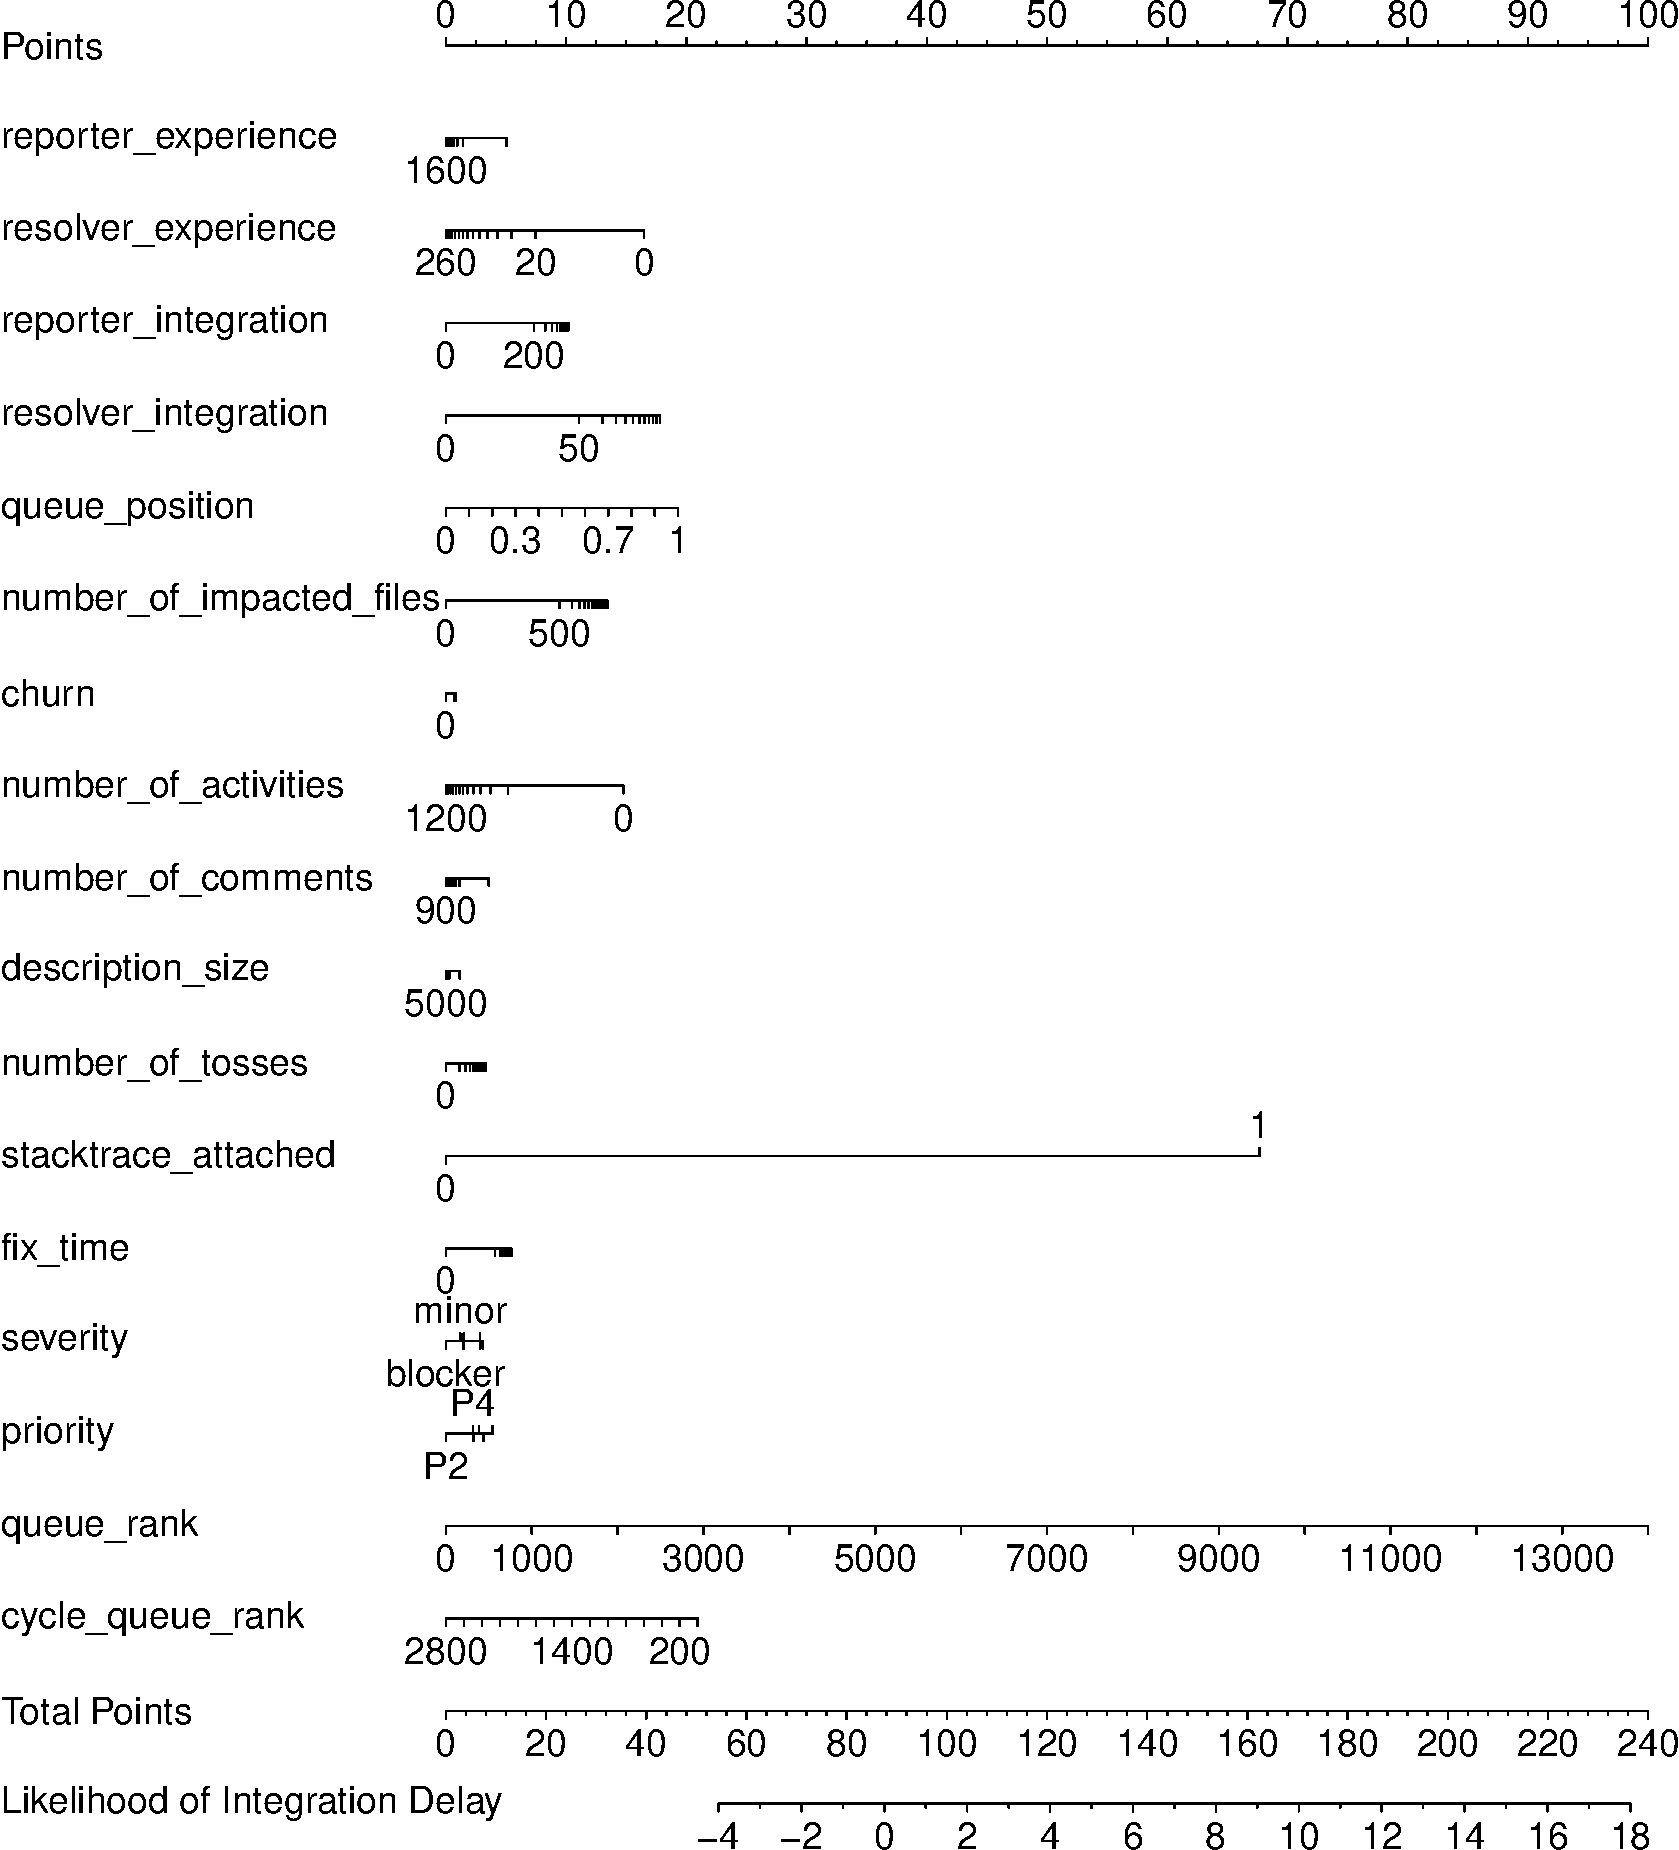
\includegraphics[width=0.90\textwidth,keepaspectratio]
	{chapters/chapter5/figures/rq3/nomogram_trad.pdf}
	\caption{Nomogram of our explanatory models for the traditional release cycle.}
	\label{fig:nomogram_trad}
\end{figure}

\begin{figure}[!]
	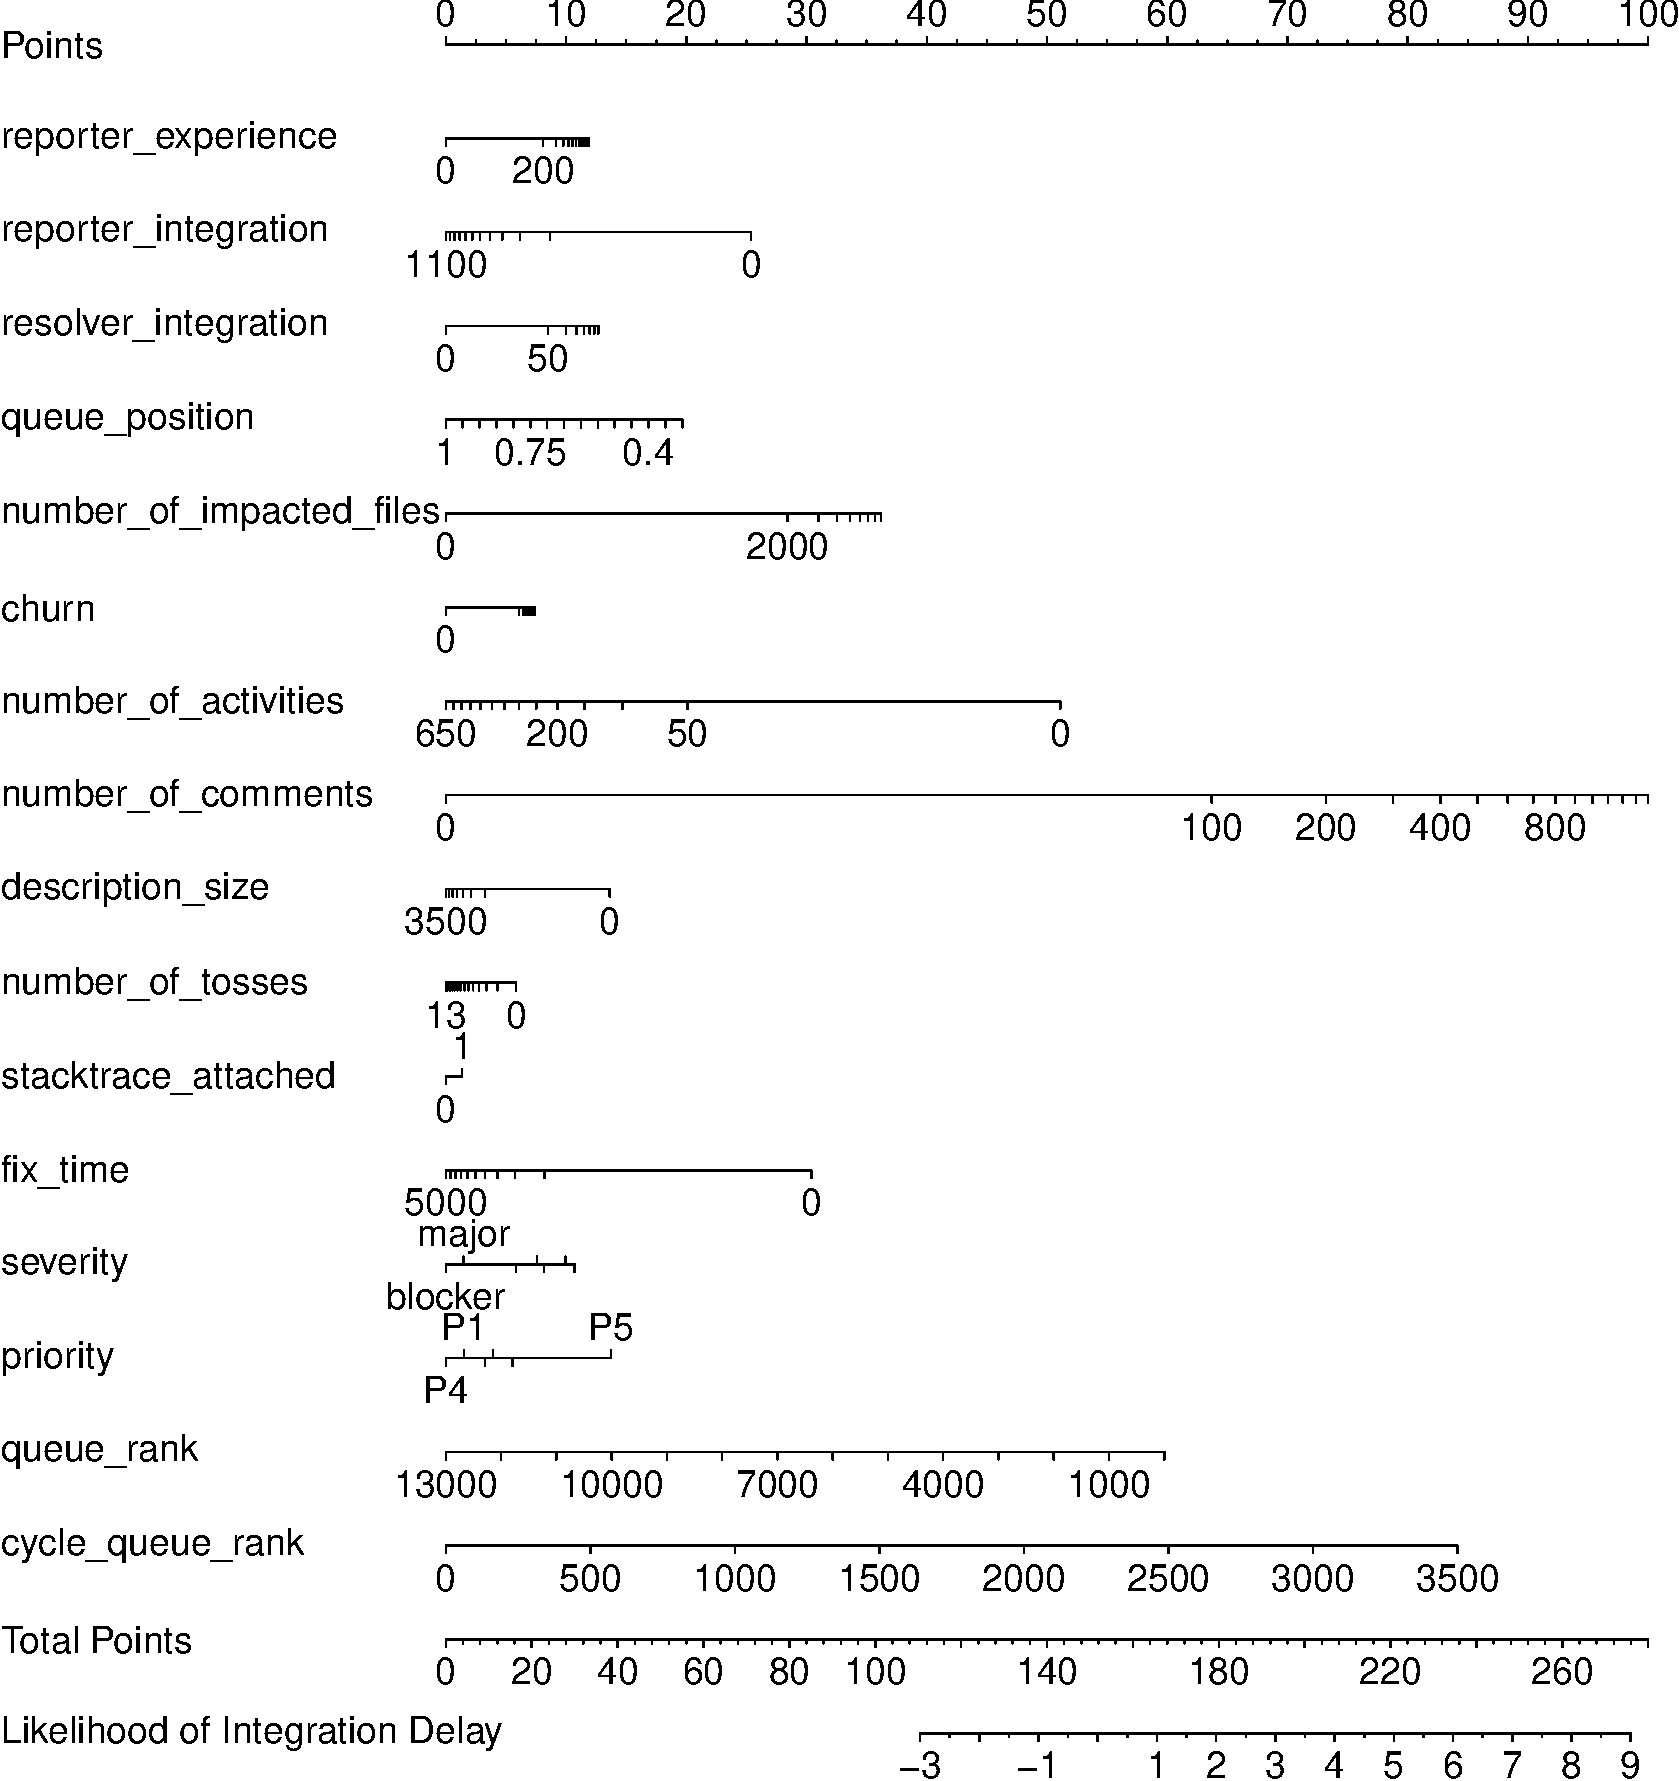
\includegraphics[width=0.90\textwidth,keepaspectratio]
	{chapters/chapter5/figures/rq3/nomogram_rapid.pdf}
	\caption{Nomogram of our explanatory models for the rapid release cycle.}
	\label{fig:nomogram_rapid}
\end{figure}

On the other hand, \textit{cycle queue rank} is the second-most important metric
in the models that we fit to the rapid release data. Cycle queue rank is the
moment when an issue is addressed in a given release cycle.
\hyperref[fig:cycle_rank]{Figure}~\ref{fig:cycle_rank} shows the relationship that cycle queue rank shares
with delivery delay. Our models reveal that the addressed issues in rapid
releases have a higher likelihood of being delayed if they were addressed later
than other addressed issues in the \textit{current release cycle}.
Interestingly, we observe that the most important metric in our rapid release
models is the \textit{number of comments}.
\hyperref[fig:number_comments]{Figure}~\ref{fig:number_comments}
shows the relationship that the \textit{number of comments} shares with
delivery delay. We observe that the greater the number of comments of an
addressed issue, the greater the likelihood of delivery delay. This result
corroborates the intuition that a lengthy discussion might be indicative of a
complex issue, which may be more likely to be delayed.

Moreover,
\hyperref[fig:nomogram_trad]{Figures}~\ref{fig:nomogram_trad}~and~\ref{fig:nomogram_rapid}
show the estimated effect of our metrics using
nomograms~\cite{iasonos2008build}. Indeed, our nomograms reiterate the large
impact of \textit{number of comments} (100 points) and \textit{cycle queue rank}
(84 points) in rapid releases, and the large impact of \textit{queue rank} (100
points) in traditional releases.  We also observe that \textit{stack trace
attached} has a large impact on traditional releases (68 points) despite not
being a significant contributor to the fit of our models (\cf
\hyperref[tbl:regression_models]{Table}~\ref{tbl:regression_models}). The large
impact shown in our nomogram for \textit{stack trace attached} is due to the
skewness of our data---only $5$ instances within the traditional release data
have the \textit{stack trace attached} set to true. Thus, \textit{stack trace
attached} cannot significantly contribute to the overall fit~of~our~models.

Another \textit{key} difference between traditional
and rapid releases is how addressed issues are prioritized for delivery.
Traditional releases are analogous to a queue in which the earlier an issue is
addressed, the lower its likelihood of delay. On the other hand, rapid
releases are analogous to a stack of cycles, in which the earlier an issue is
addressed in the current cycle, the lower its likelihood of delay.\\
\end{sloppypar}

\conclusionbox{Issues that are addressed early in the
	project backlog are less likely to be delayed in traditional releases.
	On the other hand, issues in rapid releases are queued up on a per
	release basis, in which issues that are addressed early in the release
cycle of the current release are less likely to be delayed.}

